\chapter{Installations and datasets}

\begin{figure}[h]
\centering
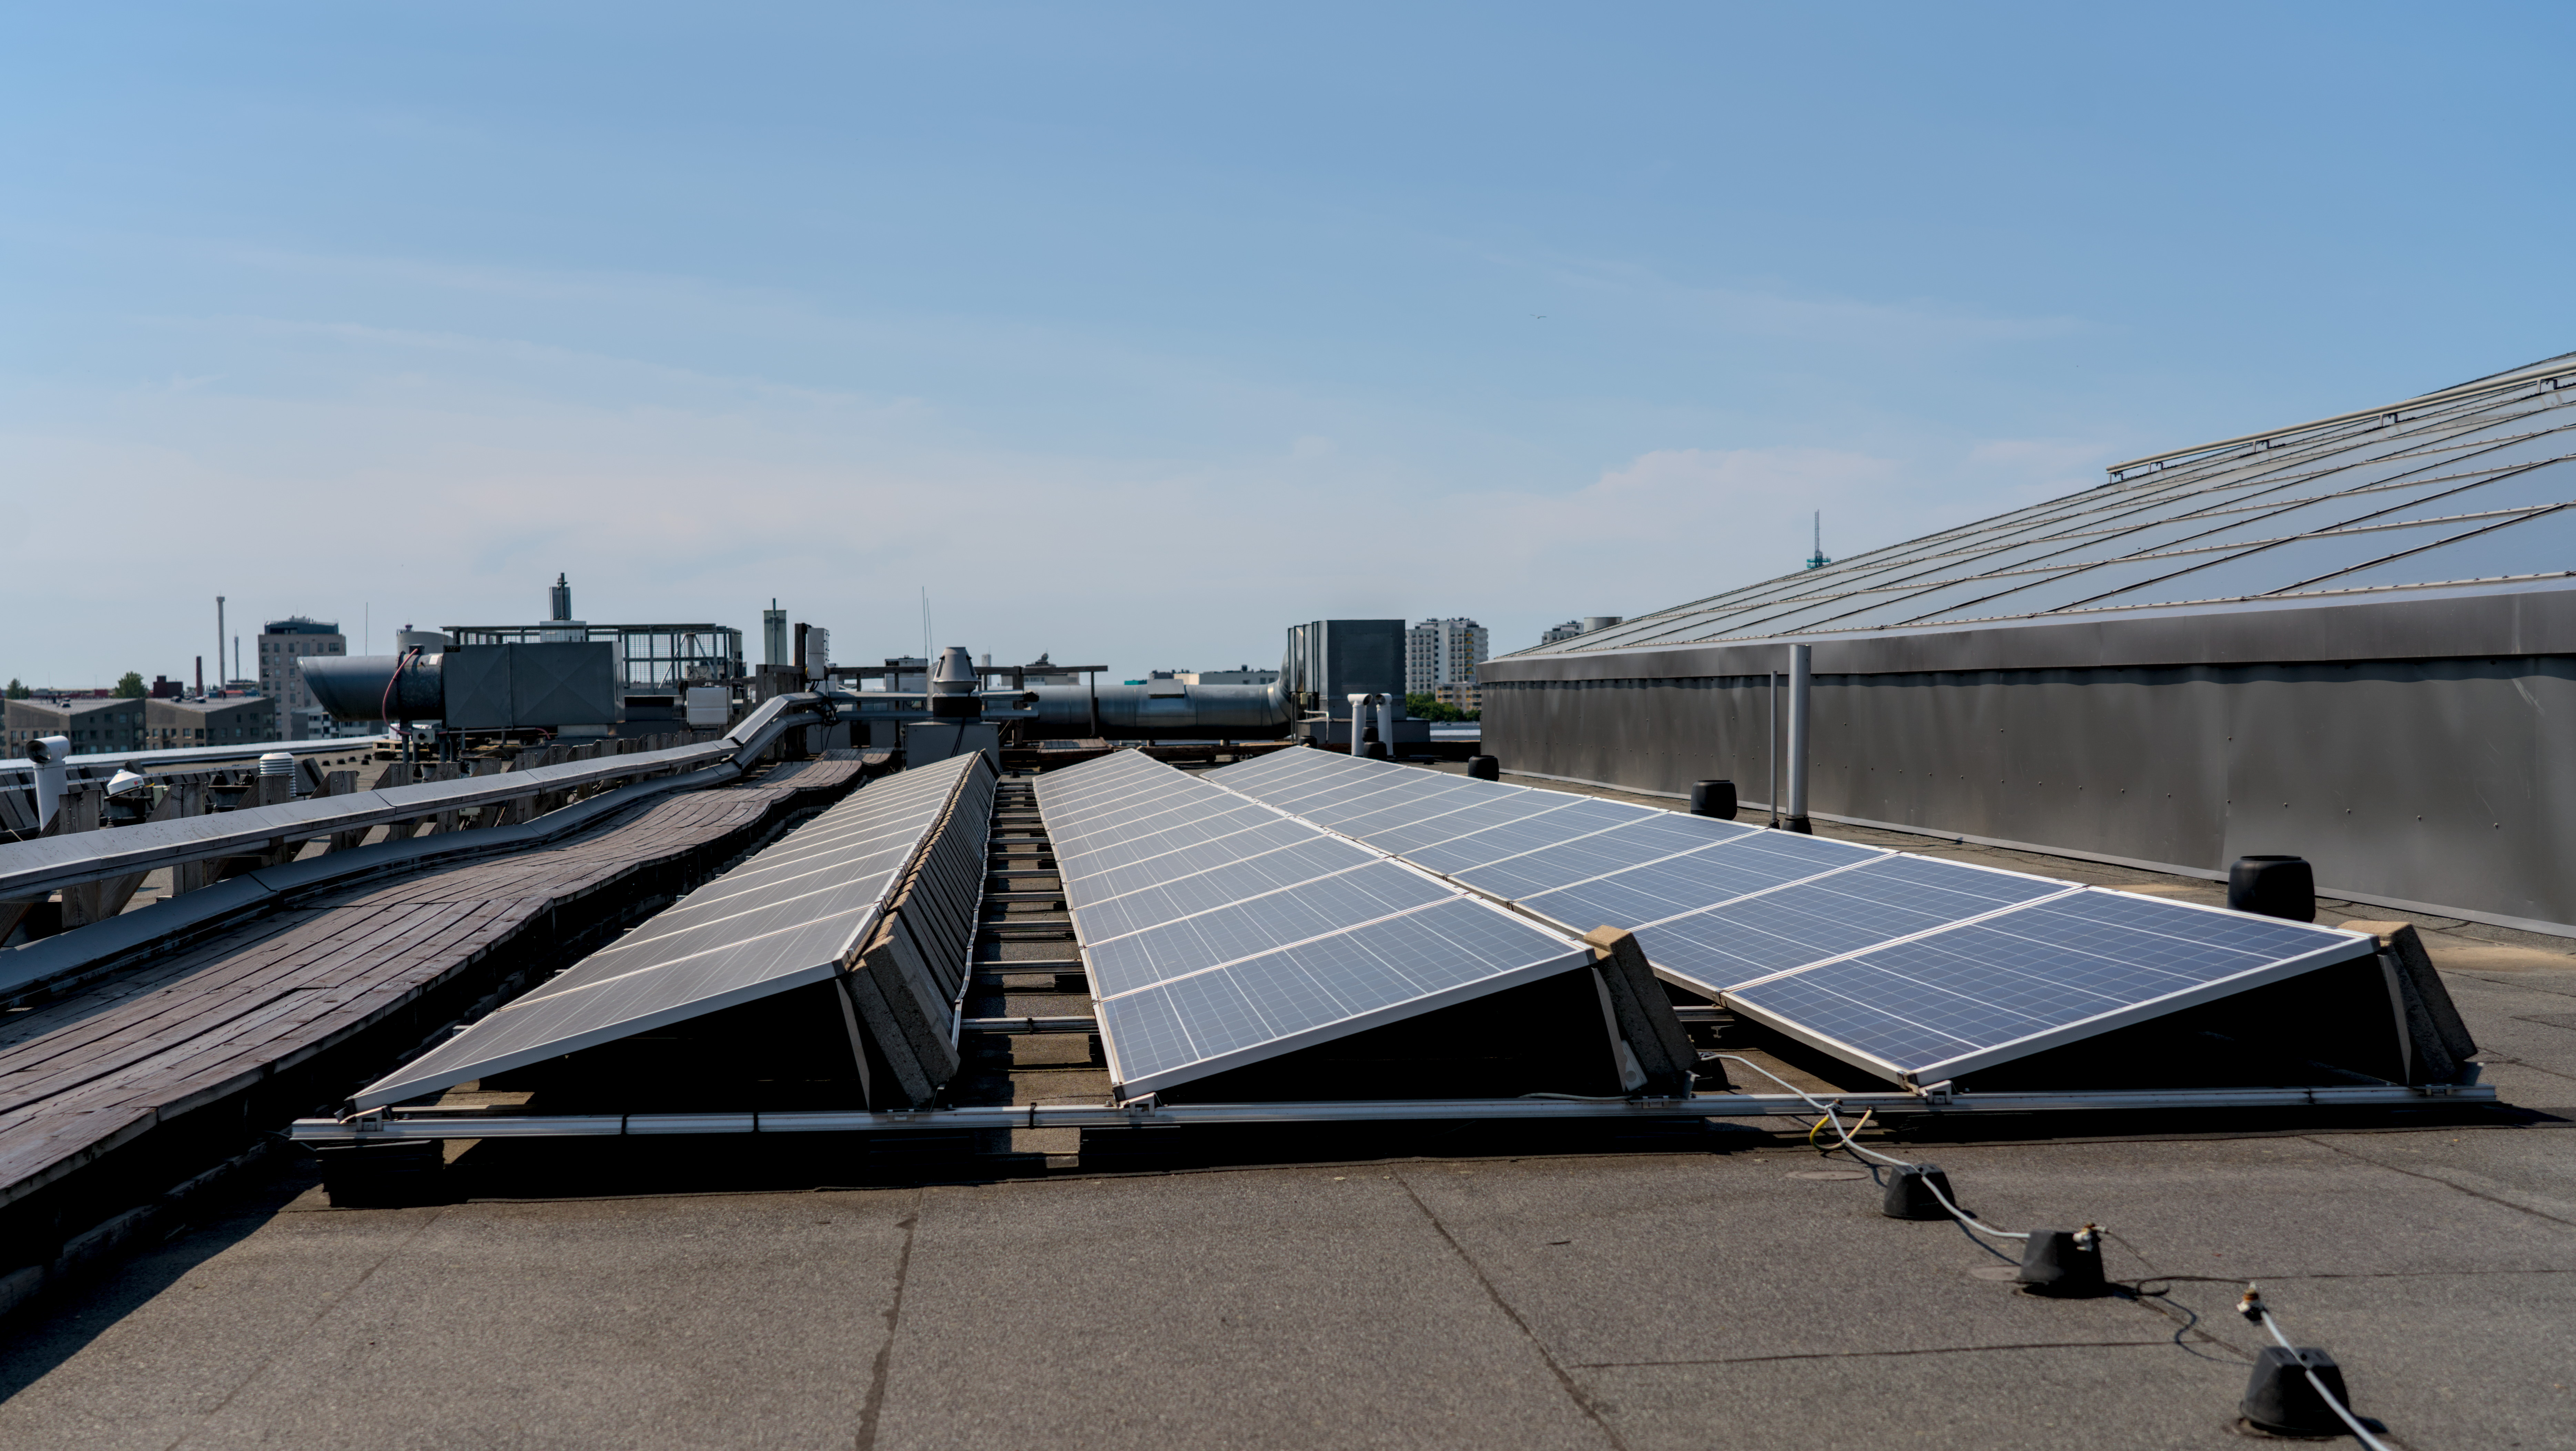
\includegraphics[width=0.8\linewidth]{pics/fmikumpula}
\figcaption{FMI Kumpula solar power installation string.}
\label{fig_fmikumpula_panels}
\end{figure}


\noindent The two datasets used in this thesis were provided by FMI. They contain power generation measurements from installations in Kuopio and Helsinki, with the physical parameters listed in table \ref{table_fmi_helsinki_kuopio_parameters}. Due to the high elevation of the installations, shading is unlikely to be a major factor in either of the datasets. The same data was previously used in Herman Böök's \textit{Photovoltaic output modeling}\cite{hbook1} and thus installation parameters and datasets have previously been verified.

The data in the two datasets follows the structure seen in table \ref{table_fmi_kumpula_csv}. This snapshot from the Helsinki dataset shows that the temporal resolution is one measurement per minute and that there are four power values for each minute. Power values in columns String 1 and String 2 represent power output from two identical sets of solar PV panels, one of which is shown in \ref{fig_fmikumpula_panels}. Electricity generated by these sets of solar panels is fed into the inverter and thus the inverter input should match the sum of String 1 and String 2. The inverter then increases the voltage and changes the direct current to alternating current. Losses in the process should result in an inverter output value which is lower than the inverter input, but this does not appear to be true for every dataframe column. A plausible cause is the input/output measuring method which may result in noise in either input or output sides of the inverter.


Datasets from other sources may have different temporal resolutions, use different units or measuring points. From the consumer point of view, the inverter output is the useful power value and so this will be the power value used by algorithms in this thesis. Temporal resolution of the FMI data will be used as is.


\begin{table}[h]

\centering

\begin{tabular}{r|cccc} \hline\hline

Timestamp[UTC] & Inverter out & Inverter in & String 1 & String 2\\ \hline
$2015-08-26$ $03:34$ & $NaN$ & $NaN$ & $0.5$ & $NaN$\\
$2015-08-26$ $03:36$ & $11.1$ & $7.5$ & $2.6$ & $4.9$\\
$2015-08-26$ $03:37$ & $25.4$ & $26.1$ & $9.8$ & $16.3$\\
$2015-08-26$ $03:38$ & $30.7$& $NaN$ & $NaN$ & $0.4$\\
$2015-08-26$ $03:39$ & $46.4$& $44.8$ & $20$ & $24.8$\\
$2015-08-26$ $03:40$ & $3.3$ & $NaN$ & $NaN$ & $0.4$\\
$2015-08-26$ $03:41$ & $29.3$ &  $18$ & $9.1$ & $8.9$\\
$2015-08-26$ $03:42$ & $33.1$& $27.4$ & $10.6$ & $16.9$\\

\vdots & \vdots & \vdots & \vdots & \vdots\\
$2015-08-26$ $12:42$ & $12374.8$ & $14619.1$ & $7152$ & $7467.1$\\
$2015-08-26$ $12:43$ & $15442.2$ & $15482.1 $& $7708.9$ & $7773.2$\\
$2015-08-26$ $12:44$ & $14085.8$ & $12898.7$ & $6387$ & $6511.8$ \\
\vdots & \vdots & \vdots & \vdots & \vdots\\

\hline\hline
\end{tabular}

\tabcaption{A section from FMI's Kumpula solar site PV production data, only the timestamp and inverter output values are used by the algorithms in this thesis. All power measurements are in watts.}
\label{table_fmi_kumpula_csv}
\end{table}





\begin{table}[H]
\centering
\begin{tabular}{r|cc} \hline\hline

 & Helsinki & Kuopio\\ \hline
 Latitude & $60.204^\circ$ & $62.892^\circ$ \\
 Longitude & $24.961^\circ$  &  $27.634^\circ$\\
 Nominal capacity &21 kW & 20.28 kW \\
 Panel tilt & $15^\circ$ & $15^\circ$ \\
 Panel azimuth & $135^\circ$ & $217^\circ$ \\
 Elevation & 17m & 10m\\
\hline\hline
\end{tabular}
\tabcaption{Parameters for the FMI's Kumpula(Helsinki) and Kuopio PV installations as listed in Böök 2020 \cite{hbook1}.}
\label{table_fmi_helsinki_kuopio_parameters}
\end{table}


\begin{figure}[h]
\centering
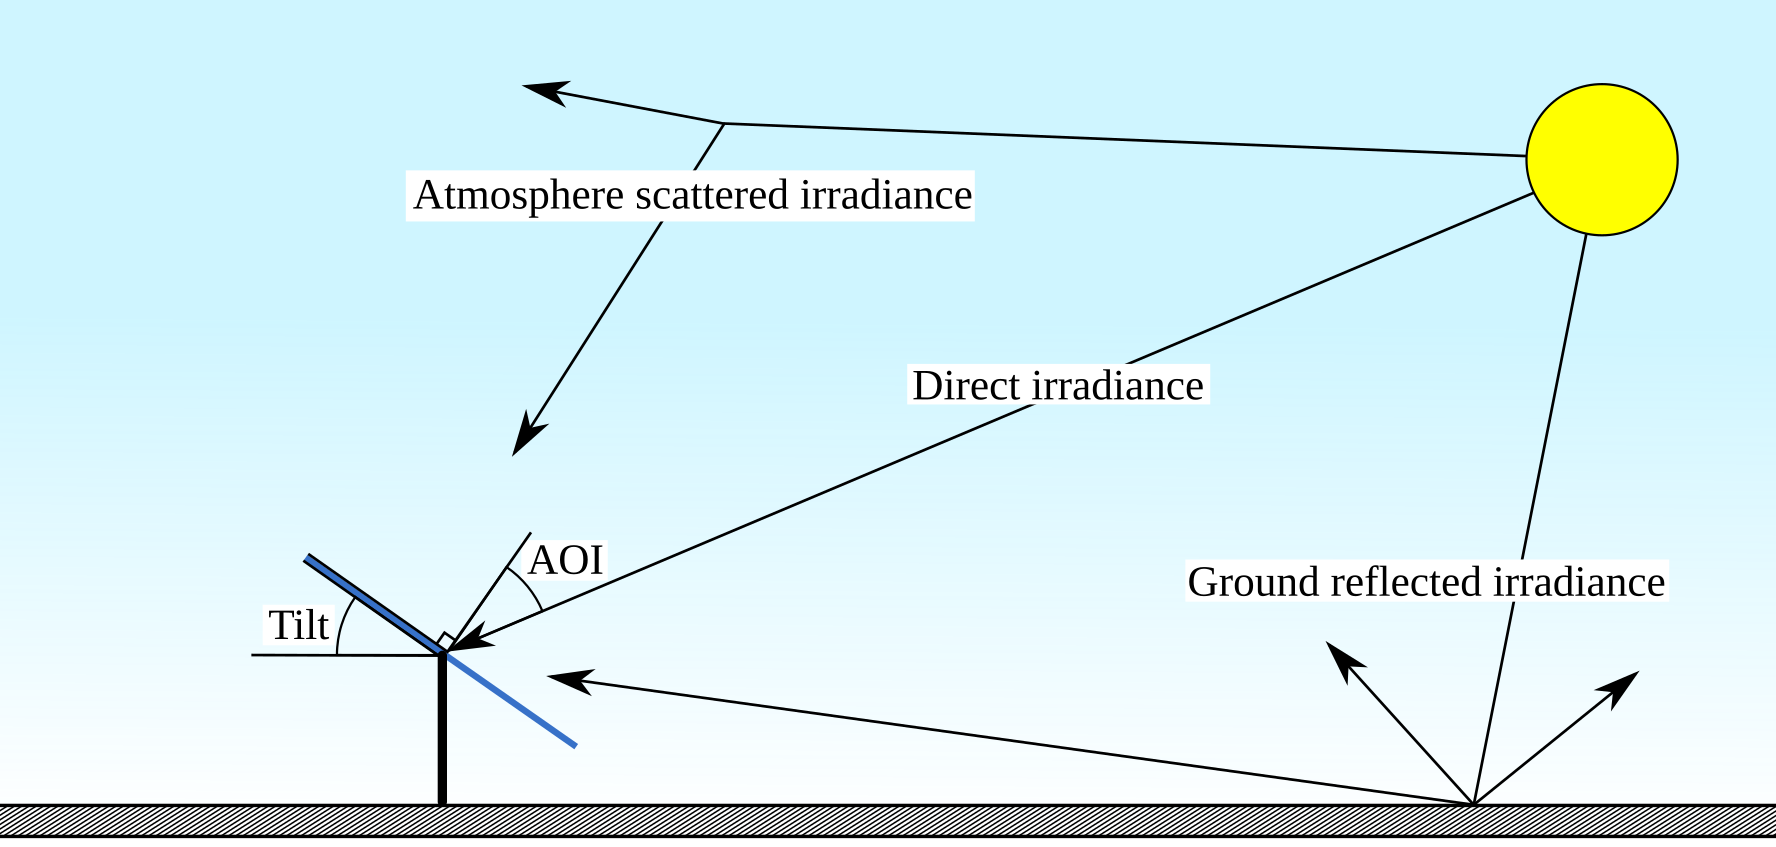
\includegraphics[width=0.8\linewidth]{pics/irradiancetypes}
\figcaption{Simplified installation diagram for a PV system in ideal conditions.}
\label{fig_simplediagram}
\end{figure}

\noindent
Figure \ref{fig_simplediagram} shows a two dimensional simplification of a solar PV installation. The abbreviation AOI stands for angle of incidence and it is defined as the angle between direct irradiance and solar panel normal. AOI can be calculated with computer programs and software libraries when geolocation, panel tilt and azimuth and the time are known. The azimuth angle is not marked on the figure and azimuth represents the second panel normal component. Azimuth for geographic north is 0$^\circ$ degrees and azimuth is measured in clockwise degrees from north. The angles given for Helsinki ($135^\circ$) and Kuopio ($217^\circ$) installations tell us that the panels are facing southeast and southwest respectively. 



\section{Visualizing the data}
The figure \ref{fig_oneyear_pointcloud} contains a 3D point cloud generated by plotting one year of data from FMI Helsinki dataset and it shows that there are visible structures in the data. The clearest structure in the 3D plot is the pattern formed by the first and last non-zero power minutes and this is later used for geolocation estimation. The second pattern is the dome-like shape of the point cloud. This shape can be examined by taking one day slices from the dataset and plotting them individually as shown in \ref{fig_cloudfree_vs_cloudy}. These slices are used for panel installation angle estimation.

\begin{figure}[h]
\centering
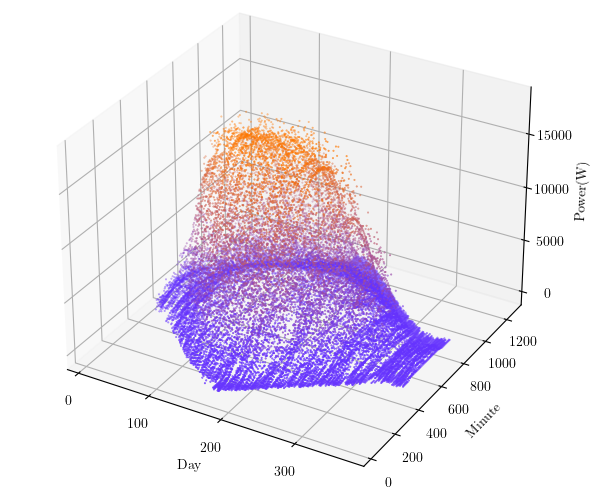
\includegraphics[width=0.8\linewidth]{pics/oneyear2}
\figcaption{One year of data from FMI Kumpula installation as a 3D point cloud.}
\label{fig_oneyear_pointcloud}
\end{figure}

\newpage
\begin{figure}[h!]
\centering
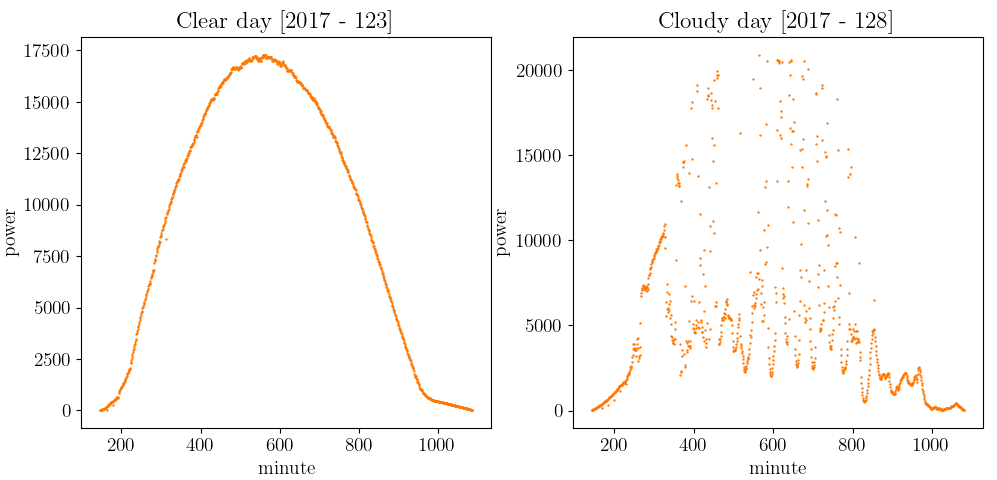
\includegraphics[width=1\linewidth]{pics/cloudfree_vs_cloudy}
\figcaption{Two days from FMI Kumpula dataset with different charasteristics.}
\label{fig_cloudfree_vs_cloudy}
\end{figure}

\noindent The presumably cloud free day 2017-123 in \ref{fig_cloudfree_vs_cloudy} has some notable charasteristics in addition to the geolocation derived first and last minutes. The shape resembles a right skewed normal distribution with a knee section near 950 minutes. As the absorbed irradiance of a PV system consists of direct and indirect irradiance, this knee section is likely to signify the point in time at which angle of incidence reaches 90 degrees.

Another measurable trait is the peak power generation minute. Geometric intuition would suggest that this should align with the moment in time with the lowest angle of incidence but this relationship could be fairly complex due to temperature induced efficiency variation and atmopshere induced losses which are higher when the Sun elevation is low.



%Note that this transition appears to be smooth and this may be a result of high reflective losses at high AOI. Similarly, intuition would suggest that the peak power minute occurs when the angle of incidence is at its minimum. Measurable traits such as these could have uses for parameter estimation.
%be used for parameter estimation, but the relationships between figure traits and system parameters can be complicated.


\newpage
\section{Data pre-processing}
The data pre-processing required by the algorithms in this thesis can be split into two gategories, classifying preprocessing and reparing preprocessing. Classifying preprocessing is used to determine if a certain section of data is useful of analysis or not, the primary example here is the cloud free day detection algorithm which is discussed more throroughly in the next chapters. The second type of preprocessing, reparing preprocessing refers to the use of algorithms which fill gaps measurement data or otherwise attempt to repair data which is unusable as is, but which could be used after repairing.

The data preprocessing algorithms used in this thesis load the data from csv files and examine whether individual days in the dataset meet set qualification requirements. These are the minimum and maximum measurement count, whether first and last measurements are taken too close to minute 0 or 1440 and the the percentage of measurements included between the first and last measurement. Figure \ref{fig_accepted_days} contains a comparison on which days in the datasets met the requirements.


\begin{figure}[h]
	
     \centering
     \begin{subfigure}[b]{0.48\textwidth}
         \centering
         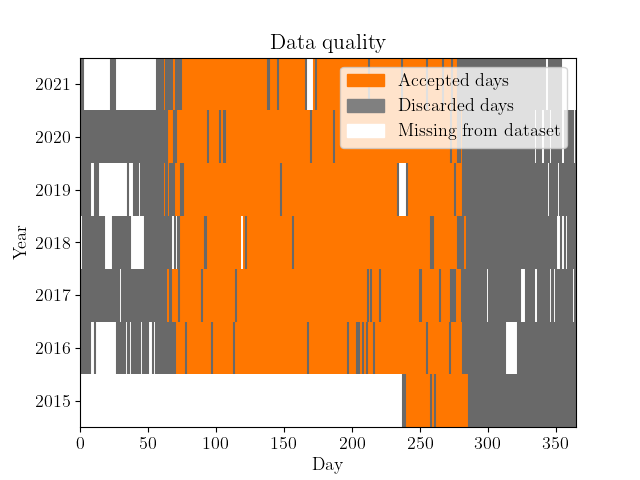
\includegraphics[width=\textwidth]{pics/helsinki_accepted_days}
         \caption{Days in Helsinki dataset which met data quality thresholds.}
         \label{fig_helsinki_accepted}
     \end{subfigure}
     \hfill
     \begin{subfigure}[b]{0.48\textwidth}
         \centering
         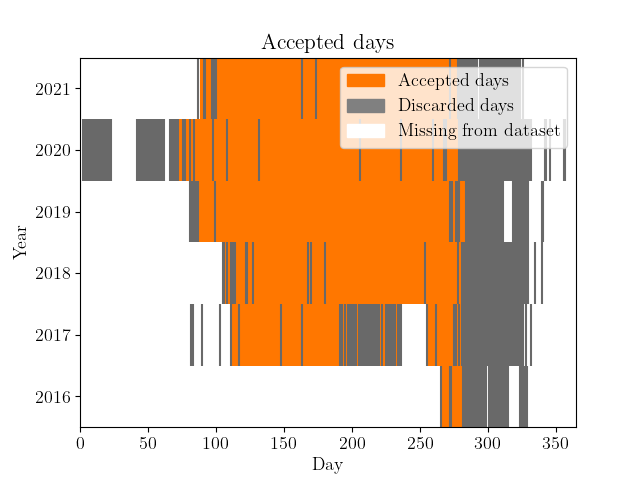
\includegraphics[width=\textwidth]{pics/kuopio_accepted_days}
         \caption{Days in Kuopio dataset which met data quality thresholds.}
         
         \label{fig_kuopio_accepted}
     \end{subfigure}
     \hfill
     \caption{Requirements were measurement count between 400 and 1200, first minute is 5th or later, last minute is 1435 or earlier. More than 95\% of measurements between first and last minute must be included.}
     \label{fig_accepted_days}
     
\end{figure}


\noindent After classification has discarded days which did not meet the set requirements, the next step is data repairing. The accepted days still contain a small amount of missing measurements and Nan values which can be linearly interpolated, meaning that if a power measurement or a set of measurements is missing between two known datapoints, the missing datapoints are estimated to describe a linear transition breaching the gap between the known datapoints. When noise is low, linearly approximating the missing values is unlikely to result in signficant errors. After this is done, the resulting data is ready for analysis.



\section{Clear day detection algorithm}
\label{clearskyalgo_chapter}
While previous preprocessing steps have filtered and repaired days according to measurement counts and data gaps, these algorithms did not filter days based on the amplitude noise present in power measurements. This power noise is typically induced by clouds and the resulting power generation curves can not be reliably used for curve fitting. The following algorithm steps can be used for automating the process of selecting days with minimal high-frequency fluctuations.


% If the interference in measurements caused by clouds or other sources is significant, the value of a day for model fitting is reduced. An example of strong interference can be seen in figure \ref{fig_cloudfree_vs_cloudy}. Detecting the presence of such interference with an algorithm would help with automating the process of model fitting as that would eliminate the need to manually select good days from datasets. The following steps describe the process used for cloud free day detection in this thesis.



%\noindent \textbf{Algorithm step by step:}

\begin{enumerate}
  \item Split dataset into individual days based on utc timestamps.
  
  \item Create a copy of the power measurements for each day and process this copy with a low pass filter algorithm.

  
  \item Calculate the difference between the original power values and the filtered power values. This delta value increases when high-frequency noise is present.
  
  
  \item Discard days with a delta value higher than a set threshold.
  

\end{enumerate}



\noindent The mathematically non-trivial parts here are threshold selection, difference measurement and low-pass filtering. Low-pass filtering is a term borrowed from the field of signal processing, and it refers to any algorithm that removes frequencies higher than a given limit from a signal, allowing lower frequencies to pass. 



Here the filtering is done with discrete Fourier transformations (DFT) and inverse discrete Fourier transformations (IDFT). When a list of numbers is used as the input of DFT, the output is a list of ordered complex numbers, each of which represents a sine wave of a certain frequency, phase and amplitude. The sum of these wave equations forms a continuous approximation of the input values and by sampling the continuous representation, the continuous trigonometric approximation can be transformed back into discrete values. However if the complex numbers are adjusted before the IDFT operation, frequencies can be selectively modified. This means that DFT and IDFT can be used for frequency specific modification of numerical lists, low-pass filtering being one of the possibilities. In this case the low-pass filtering was accomplished by zeroing out complex numbers which do not correspond to the 6 longest frequencies, the resulting smoothening can be seen in figure \ref{fig_cloudfree_algo}.


While this process is somewhat complicated, Fourier transformations are not the only tool for creating low pass filters. Similar results can also be achieved by locally averaging each power value to be the average of nearest $k$ values. Discrete Fourier transformation based methods do however have an advantage in their universality. If the 6 or 7 or $n$ longest frequencies can be determined to be a good low-pass filter for PV power measurements, then these same frequencies should result in similar outputs no matter the temporal resolution of the power measurement data. Where as a method based on local averages would require a different window size depending on measurement intervals.

The second component is not as complicated as the low pass filtering operation. Measuring the delta between a filtered and unfiltered set of measurements can be done by computing the discrete curve length or as was done here, measuring the absolute average deviation between filtered and unfiltered power measurement as per equations \ref{eq2-1}-\ref{eq2-5}.


\begin{align}
Power &= [p_0, p_1, p_2, \dots , p_n]   \label{eq2-1}\\ 
Power_{filtered} &= [f_0, f_1, f_2, \dots , f_n] \\
Power_{delta} &= [|p_0 - f_0|, |p_1-f_1|, |p_2-f_2|, \dots , |p_n-f_n|] \\
delta_{avg} &= avg(Power_{delta}) \\
delta_{norm} &= delta_{avg}/ max(Power) \label{eq2-5}
\end{align}


\noindent The final component is threshold selection. The intermittent value $delta_{avg}$ describes the average wattage difference between measured and low pass filtered measured power values. By definition, this delta value is dependent on noise and installation size, limiting its usability. A noise only -delta value can be calculated by normalizing the delta with the $max(Power)$. The resulting $delta_{norm}$ should now be comparable between installations of different sizes. Choosing to reject every day for which $delta_{norm}$ value is higher than 0.05 would eliminate days with higher than 5\% normalized noise.




\begin{figure}[h]
\centering
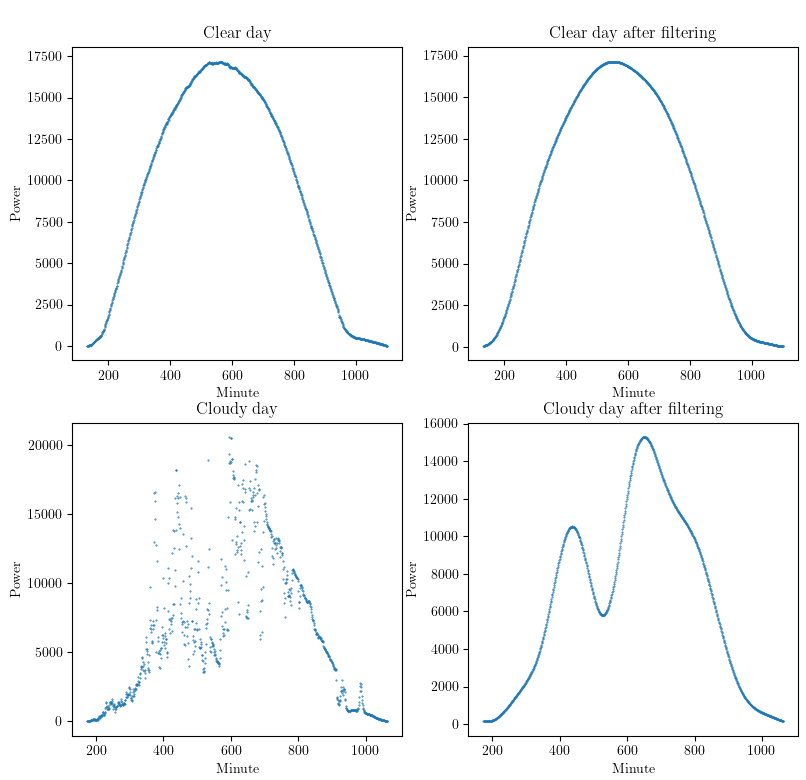
\includegraphics[width=0.8\linewidth]{pics/cloudfree_algo}
\figcaption{Cloud free day finder low pass filtering phase.}
\label{fig_cloudfree_algo}
\end{figure}



\newpage






%\noindent \textbf{Note:} that the algorithm listed above is highly dependent on measurement intervals and further tuning could be needed when operating with datasets that have different temporal resolutions. And as is, the algorithm selects days based on their proportionally low high frequency component, thus in theory this algorithm should classify zero power output days as cloud free days. Despite this fault the algorithm seems to work well for the FMI datasets.% as long as the input are selected to contain days close or between the spring and fall equinoxes. 



%The implementation of the clear sky algorithm seems to work well as indicated by \ref{fig-multidaypoavsmeasurements} but there are a few weak points in the algorithm as well. For example if a constant power day is given as the input for the algorithm, the algorithm will classify it as clear sky day even if a constant power day is more likely to be the result of faulty measuring instruments or errors in data preprocessing than a real cloud free day. In addition, the algorithm is unlikely to work well if sections are either removed from the measurements or if there is significant shading affecting the power output of the installation.

%\subsection{Difference between solar days and UTC days}
%For solar power analysis the concept of solar days is fairly useful. Solar days and sun based time measurement systems tend to rely on the angle of the sun and three 


%The timestamps used in solar PV measurements can be assumed to be in UTC +0 time. While this means that timezones or daylight saving time do not have to be accounted for, some operations may become more complicated as well since UTC days and solar days at do not always align. Note that here local solar day is defined as the 

%For example, if a one day slice is taken from a $0^\circ$ longitude installation power generation data, it is rather likely that the solar power generation would occur during an interval which centers around noon or 720 minutes. If the same slice is taken at $90^\circ$ longitude, this generation would be shifted by approximately 360 minutes. This is perfectly normal and expected behavior, but as a result, determining the first and last non-zero minutes of the day can be seen to nontrivial as per figure \ref{fig_poa0vs90}. In the $0^\circ$ plot, the first and last non-zero minutes are approximately 330 and 1100, but should the first and last minutes of the $90^\circ$ plot be defined as 0 and 750, 0 and 1420, -19 and 750 or something else entirely?


%\begin{figure}[h!]
%\centering
%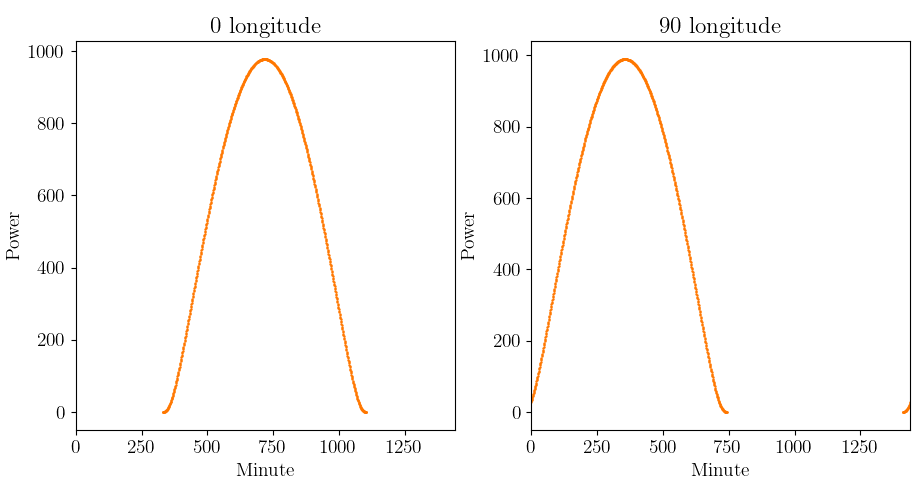
\includegraphics[width=0.9\linewidth]{pics/poa0vs90}
%\figcaption{Approximations of solar power generation at $0^\circ$ and $90^\circ$ longitude.}
%\label{fig_poa0vs90}
%\end{figure}


%\section{Third party datasets}
%Sunny portal etc here

%\section{Required assumptions}The algorithms presented in this thesis work on datasets which 


%Due to the diversity of possible solar PV installations, creating an universal model for parameter estimation is not fesiable. Installations could have been modified during operation, system failures could induce different types of changes in measurement data and 




%\section{Assumptions and possible issues}
%If metadata such as the geographic location or panel installation angles is missing from the datafiles, it is very likely that other critical pieces of information could be left out as well. Were additional modules were installed during operation? Could some panels be installed at different angles? What if the panels are installed in tracking mounts and thus the panel angles vary during each day? These questions are left unaswered and thus some assumptions have to be made. In this thesis we will assume that the panels are installed on fixed mounts, no changes were done during data gathering period and all panels are oriented similarly. We will also assume that there are no major obstacles casting shadows on the panels and that the panels are not self-shadowing, meaning that the panels are not casting shadows on one another.

%Another source of uncertainty is data collection itself. The device responsible for measuring power output values and logging the values has to have a clock for measuring time, but this clock could have be running too slow or fast, resulting in a drifting error in the timestamps. Similarly if the system clock is running at the right speed but it is off by a minute or two, this could cause a bias in the data which would be hard to detect. There is also the question of how measurement timing is done. If the time resolution of the logging device is 15 minutes, is the power value at 12:45 taken during the 45th minute or is the power value the average of the previous 15 minutes as is often done in meteorology? Or could the power value be the average of measurements taken during the interval 12:38 to 12:52? In meoteorology, the last period average would be the standard, but standards may not always be followed.

%is the standard, but standards are not always followed and thus 

%If enough time and effort was spent on algorithm design, in theory it could be possible to detect modifications to PV systems, the presence of variable panel angle systems and clock drifts. But these topics are outside the scope of this thesis and thus the assumption will be made that the 





















